%-*-    coding: UTF-8   -*-
% !TEX program = xelatex
\documentclass[UTF-8]{ctexart}
\usepackage{array}
\usepackage{graphicx}
\usepackage{float}
\usepackage{subfigure}
\usepackage{amsmath}
\usepackage{amssymb}
\usepackage{tabularx}
\usepackage{multirow}
\usepackage[usenames,dvipsnames]{color}
\usepackage{framed}
\usepackage{xcolor}
\usepackage{hyperref}
\usepackage{verbatim}
\hypersetup{
	colorlinks=true,
	linkcolor=black,
	filecolor=black,
	urlcolor=blue,
	citecolor=black,
}
\usepackage{ulem}
\usepackage[cache=false]{minted}
\setminted{tabsize=4}
\usepackage{geometry}
\geometry{a4paper,centering,scale=0.85}
\usepackage[format=hang,font=small,textfont=it]{caption}
\usepackage[nottoc]{tocbibind}

\definecolor{LightofNibel}{rgb}{0.6,0.85,0.95}
\pagecolor{white}

\title{\textbf{\huge 给信息组学弟学妹的 Linux 入门手把手教程}}
\author{\texttt{iotang}}
%\date{}

\begin{document}
	\maketitle
	
	\newpage
	
	\tableofcontents

	\newpage

	\section{欢迎使用 Linux!}
	
		学弟学妹们好!感谢你们参加信息学竞赛!
		
		比克提尼 iotang 在这里献上最诚挚的祝福!
			
		\begin{figure}[H]
			\centering
			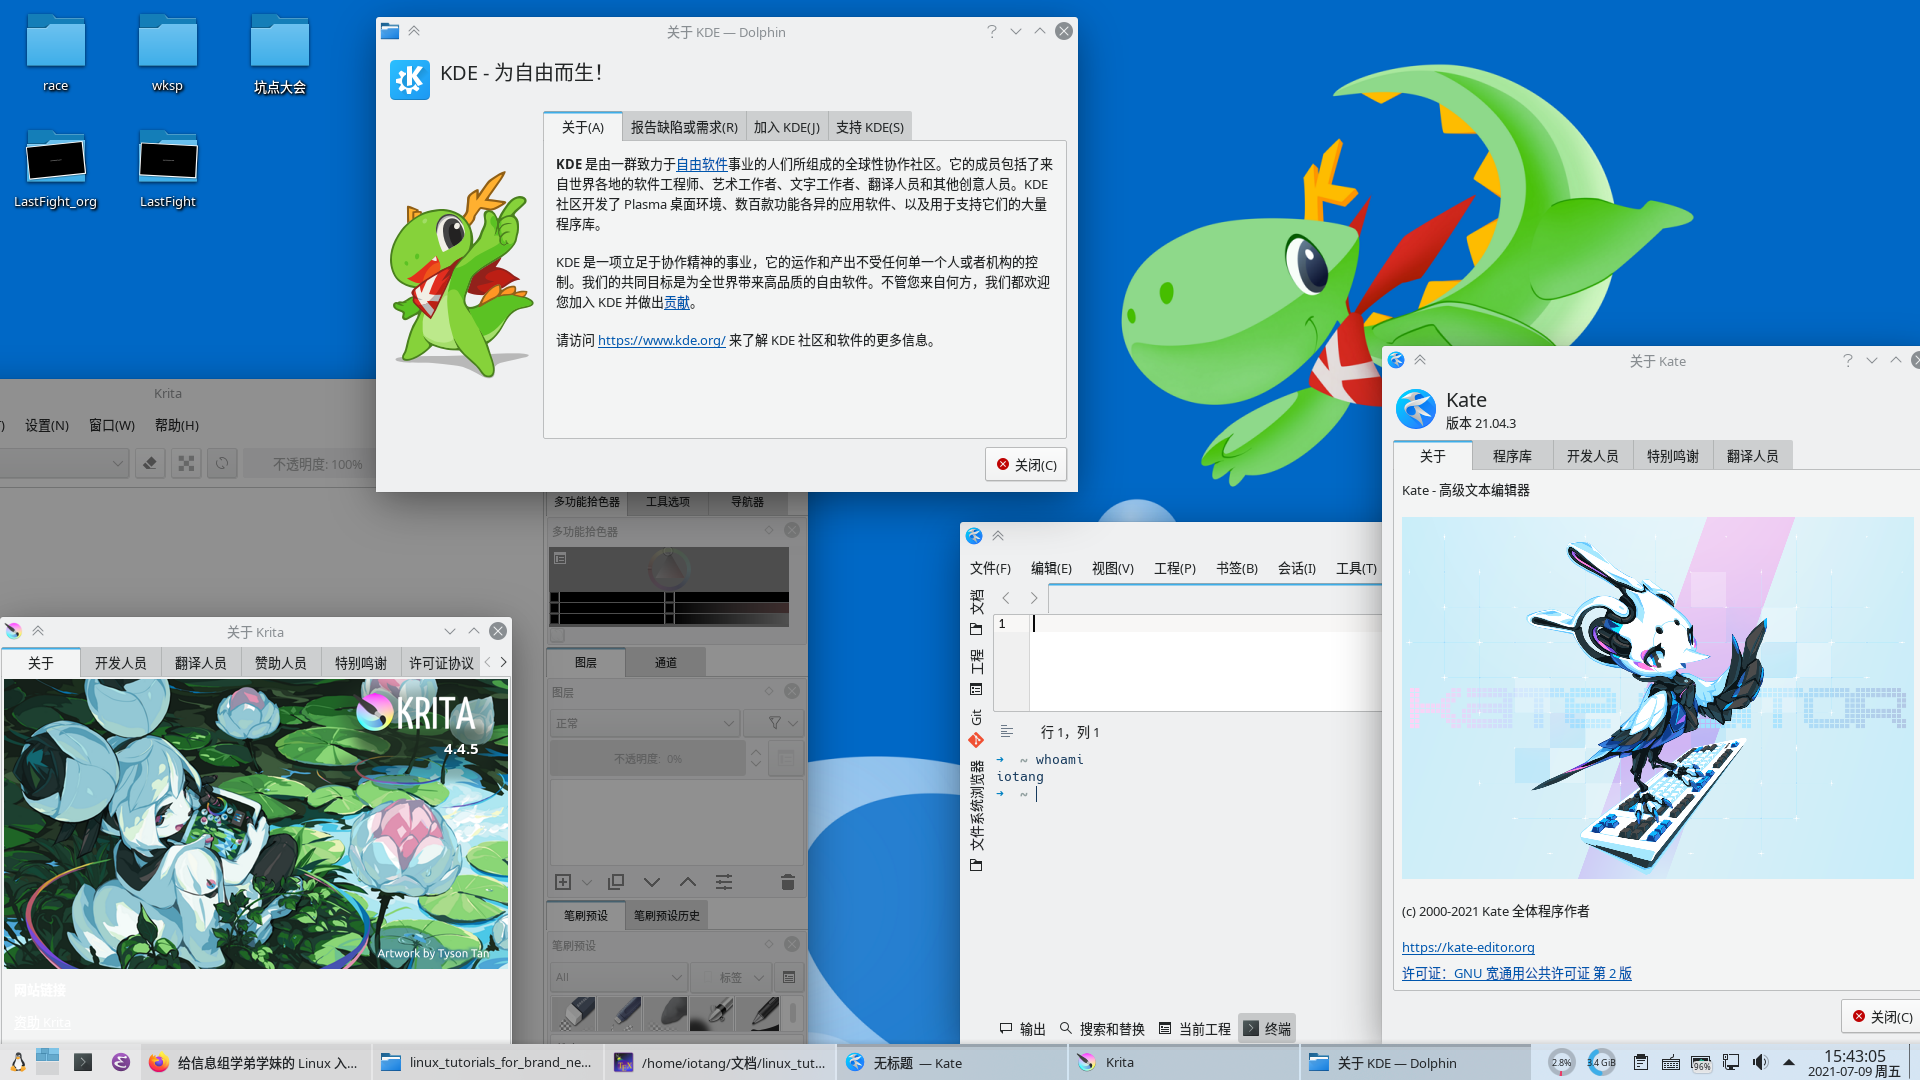
\includegraphics[width=0.8\textwidth]{fig/iotangsdesktop.png}
			\caption*{iotang 和 Konqi(左上、右上)、Kiki(左下)和 Kate(右下)向你发出问候}
		\end{figure}
	
		大家应该都对 Linux 有所耳闻,不过我猜有许多人都以为 Linux 很难用、不好用而不敢迈出第一步。
		
		现在,就让我来手把手带你们入门 Linux!
		
	\newpage
	
	\section{Linux 是开源软件}
	
		Linux 遵循 GNU 通用公共许可证,任何人都可以自由使用它的源代码。
		
		(注意,这里并没有说 Linux 是“不要钱”地使用的,不过既然你都可以搞到源代码了,那么收费基本也就没必要了。不过还是有服务以付费的方式给出。)
		
	\section{为什么是 Ubuntu?}
	
		接下来给大家带来的 Linux 教程主要是以 Ubuntu 为平台来实现的。
	
		首先很明显的是,NOI Linux 就是一个换皮的 Ubuntu。至于为什么是 Ubuntu,可能与 Ubuntu 在中国的强大的用户数量有关。
		
		用户多教程就多,问题解决也方便,\sout{不像笔者硬是要搞个 Arch Linux 然后折腾}。
		
		所以说,从竞赛与使用方面,这边还是建议大家用 Ubuntu。
	
	\newpage
	
	\section{Ubuntu 的安装}
	
		\subsection{搞到镜像文件}
		
			非常简单,你只要先百度 ubuntu,进入官网(注意:有中文官网),然后进入下载栏目下载就可以了。
			
			\subsubsection{我该选哪一个?}
			
				在下载界面你可以发现一些不同版本:
				
				\begin{figure}[H]
					\centering
					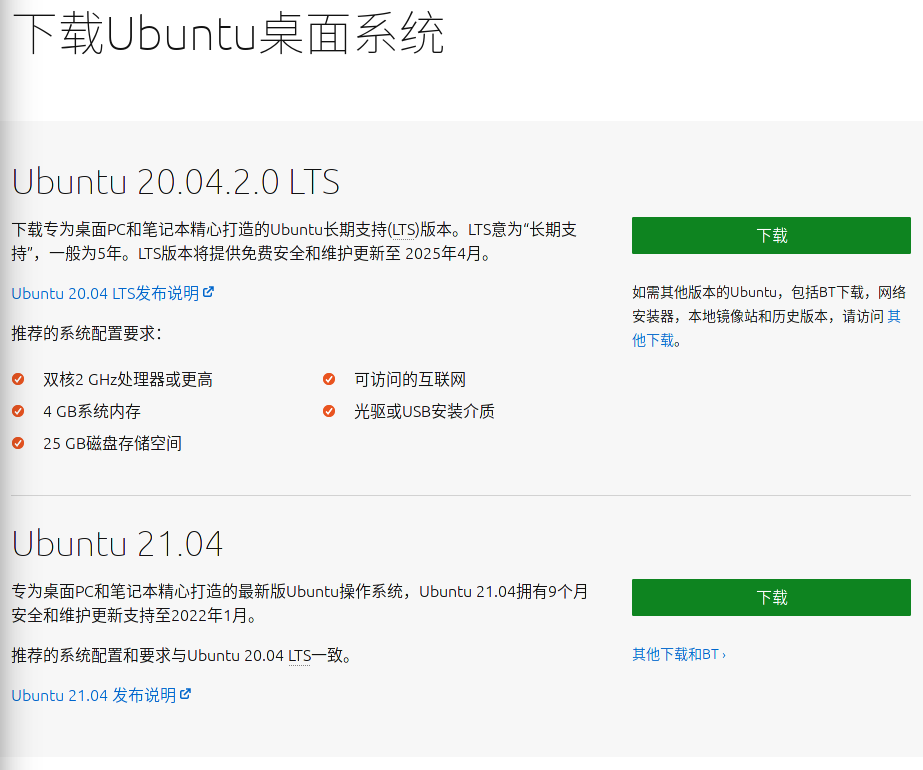
\includegraphics[width=0.8\textwidth]{fig/download_ubuntu_which.png}
					\caption*{两种选择}
				\end{figure}
			
				其中,带“LTS”的版本意为长期支持版本,有 5 年的免费安全和维护更新时间;而不带 LTS 的一般只维护 9 个月(因为不带 LTS 的每半年发布一个,你需要及时更新)。
				
				这里为了稳定性,我们下载那个带 LTS 的版本。
			
			\subsubsection{下载的速度太慢了?}
			
				你可以去其它的镜像网站。这里以网易开源镜像站为例子:
				
				首先随便搜到它的主页。
				
				\begin{figure}[H]
					\centering
					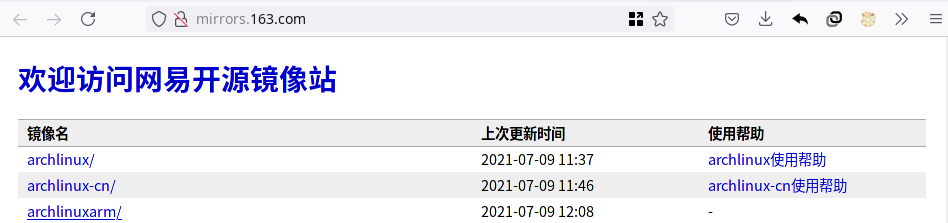
\includegraphics[width=0.8\textwidth]{fig/mirrors163com.png}
					\caption*{http://mirrors.163.com/}
				\end{figure}
			
				然后找到 \texttt{ubuntu-releases}。
				
				\begin{figure}[H]
					\centering
					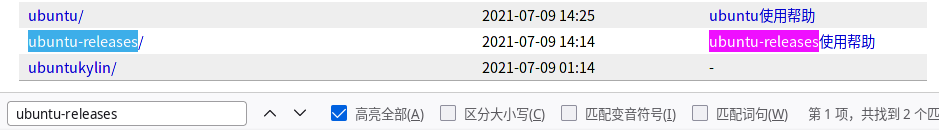
\includegraphics[width=0.8\textwidth]{fig/mirrors163com_find.png}
					\caption*{找到 ubuntu-releases}
				\end{figure}
				
				然后选择正确的版本。
				
				\begin{figure}[H]
					\centering
					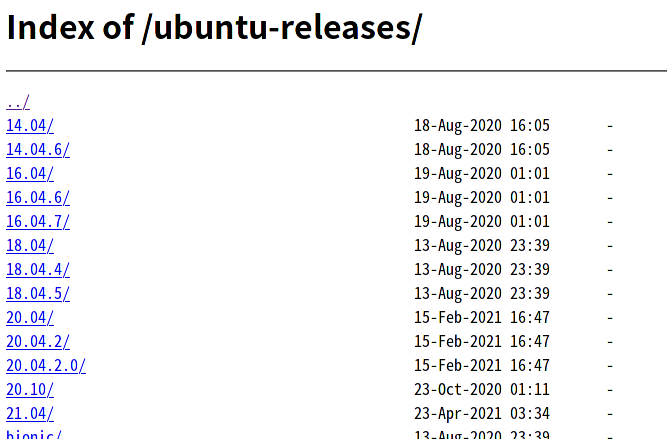
\includegraphics[width=0.8\textwidth]{fig/mirrors163com_in_ubuntu-releases.png}
					\caption*{/ubuntu-releases/}
				\end{figure}
			
				下载桌面版,即名字里面有 desktop 的那个。
				
				\begin{figure}[H]
					\centering
					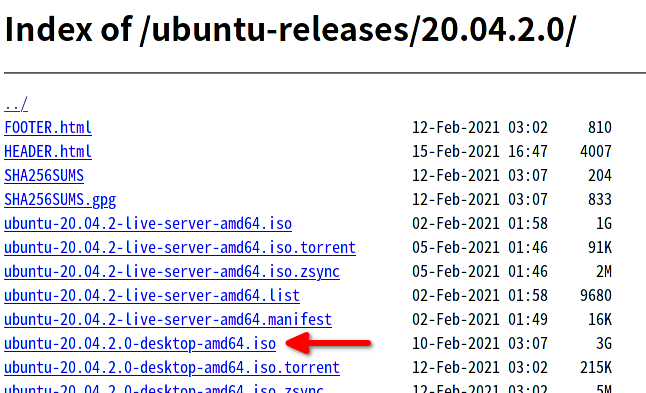
\includegraphics[width=0.8\textwidth]{fig/mirrors163com_choose_ubuntu-releases.png}
					\caption*{选择桌面版}
				\end{figure}
			
		\subsection{制作启动盘}
		
			\subsubsection{在 Linux 下}
			
				系统但凡是有点良心都会自带一个启动盘创建器。比如笔者的:
			
				\begin{figure}[H]
					\centering
					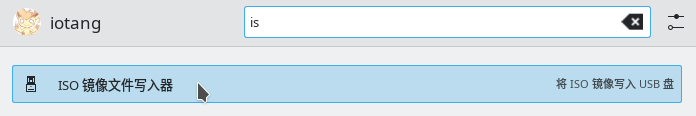
\includegraphics[width=0.8\textwidth]{fig/iso_burn.png}
					\caption*{KDE 下的启动盘创建器}
				\end{figure}
				
				此时,你需要准备一个 U 盘(最好至少 8 GB,并且笔者建议这个 U 盘应该是空的,以确保\textbf{\large 没有重要文件在里面}被抹去。)
				
				启动盘创建器的用法基本都一样。注意不要选错 U 盘。
			
				\begin{figure}[H]
					\centering
					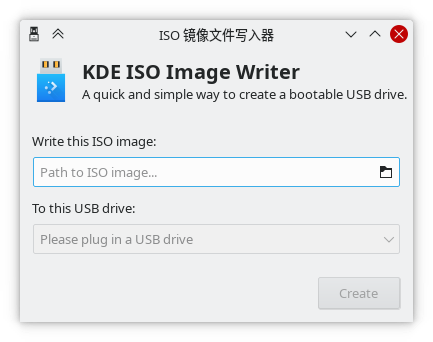
\includegraphics[width=0.3\textwidth]{fig/isoimagewriter.png}
					\caption*{KDE 启动盘创建器}
				\end{figure}


			\subsubsection{在 Windows 下}
			
				去下载 Rufus 启动盘创建器。
				
				\begin{figure}[H]
					\centering
					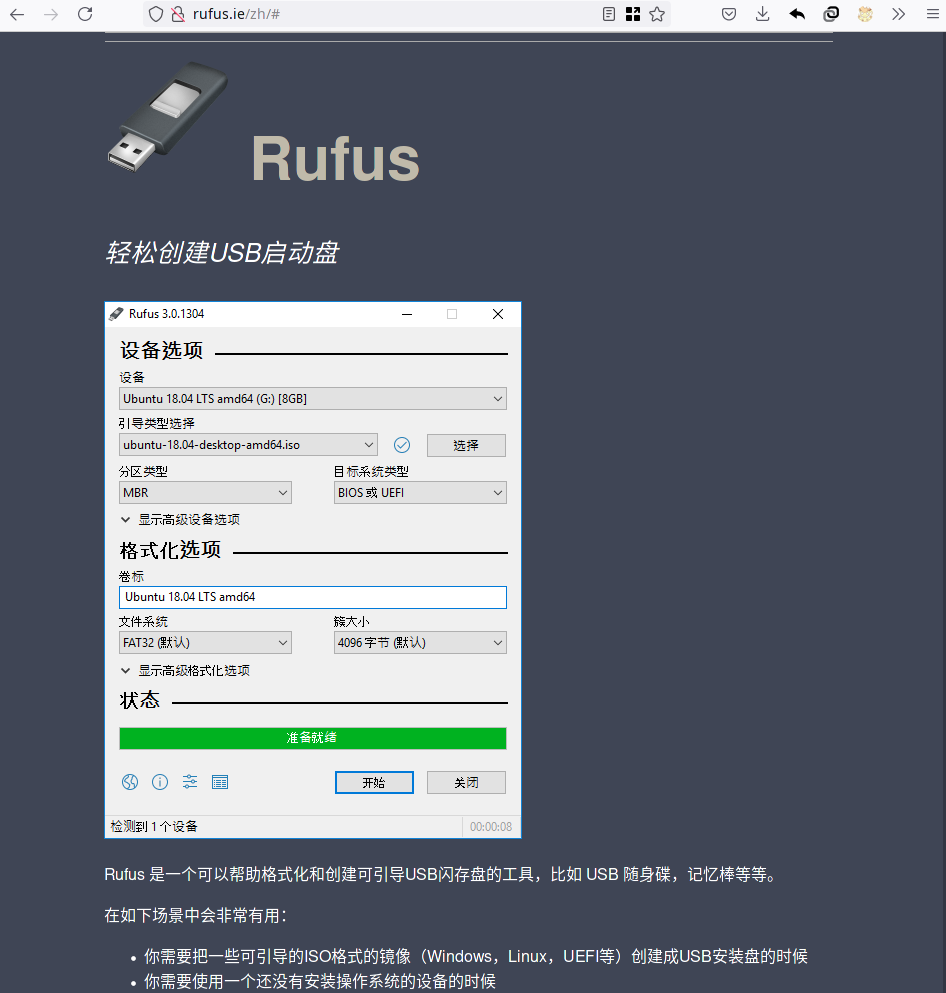
\includegraphics[width=0.8\textwidth]{fig/rufus.png}
					\caption*{Rufus}
				\end{figure}
			
		\subsection{安装 Ubuntu}
		
			我们马上会在目标电脑(机房里面的一台)上安装 Ubuntu。
		
			\subsubsection{BIOS 设置}
			
				首先打开目标电脑,在 Logo 出现后(甚至从电源键按下前)开始狂按 BIOS 键(比如 F12、ESC、DEL 等等)。
				
				在 BIOS 设置中打开 U 盘启动,打开 UEFI 模式优先(原先一般是 Legacy 优先)。
			
			\subsubsection{开始安装}
				
				关机,插上启动盘,开机后会出来一个界面让你选择启动位置。选择你的 U 盘(一般叫 USB-HDD 什么的)。
				
				之后在试用 Ubuntu 和安装 Ubuntu 中选择安装 Ubuntu。
				
				\begin{figure}[H]
					\centering
					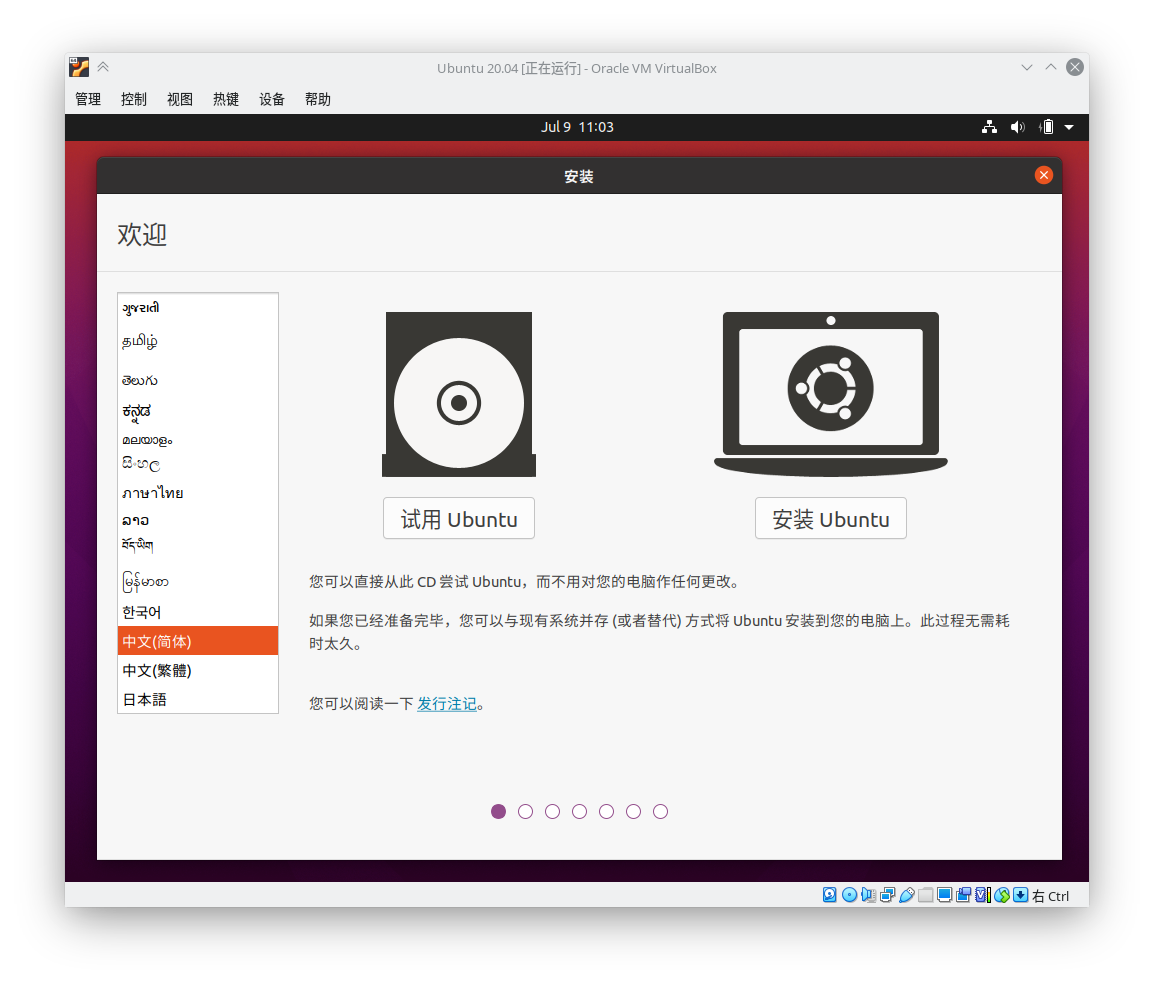
\includegraphics[width=0.7\textwidth]{fig/ubuntu_install_1.png}
					\caption*{安装 Ubuntu}
				\end{figure}
			
				选择键盘布局为 English (US)。
			
				\begin{figure}[H]
					\centering
					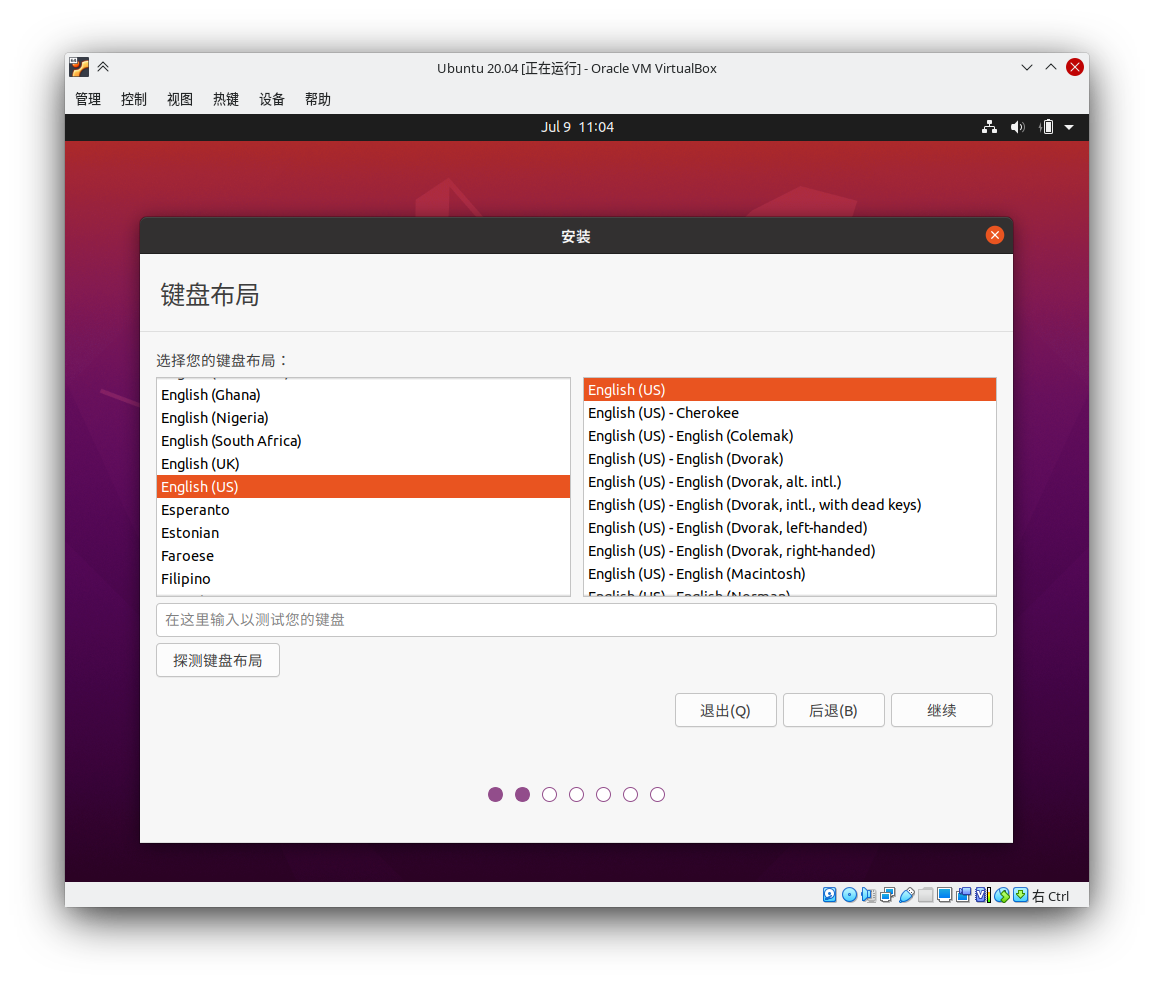
\includegraphics[width=0.7\textwidth]{fig/ubuntu_install_2.png}
					\caption*{选择键盘布局}
				\end{figure}
			
				建议先选择“最小安装”,并且不选“安装 Ubuntu 时下载更新”。
			
				\begin{figure}[H]
					\centering
					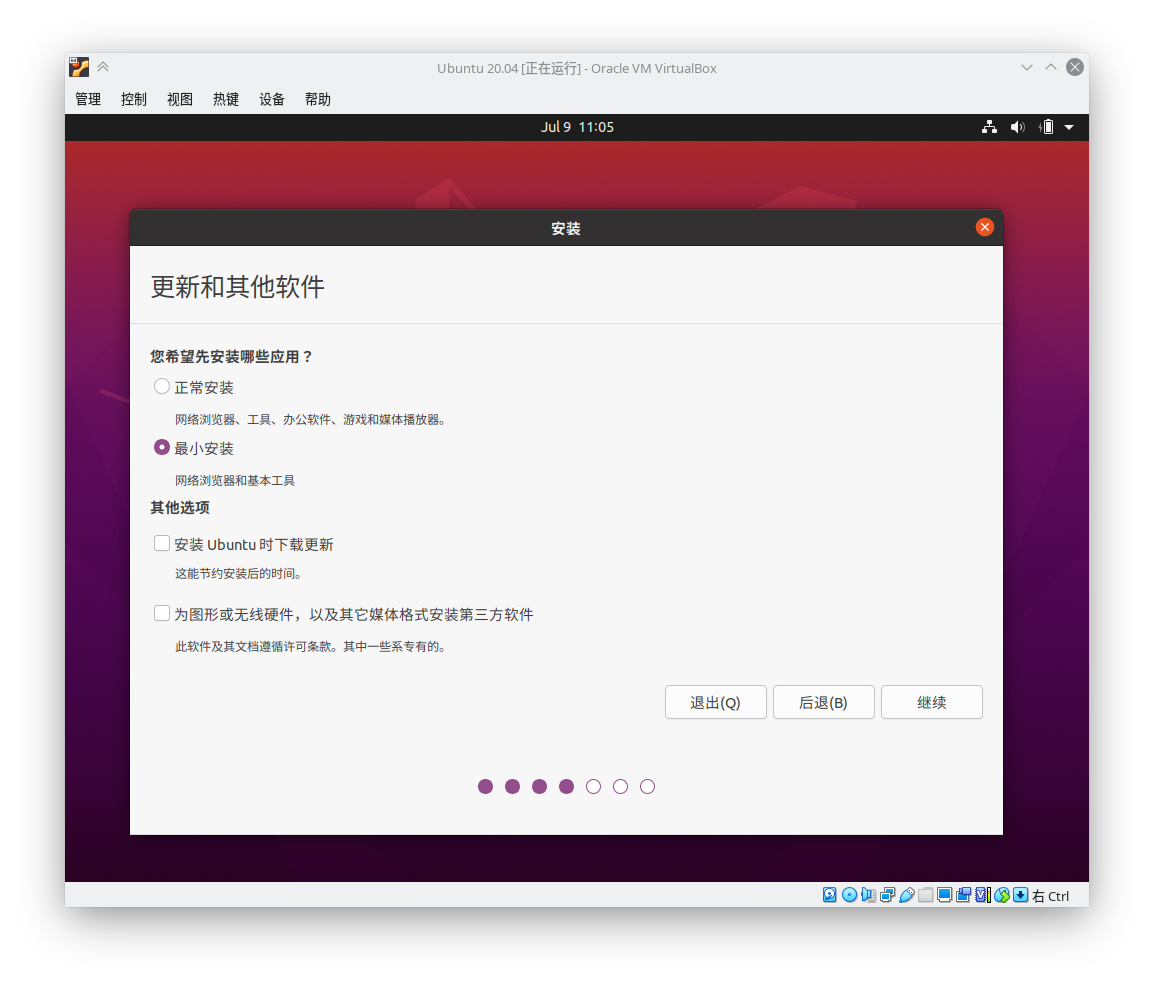
\includegraphics[width=0.7\textwidth]{fig/ubuntu_install_4.png}
					\caption*{更新和其他软件}
				\end{figure}
			
				根据需要选择安装类型。
			
				\begin{figure}[H]
					\centering
					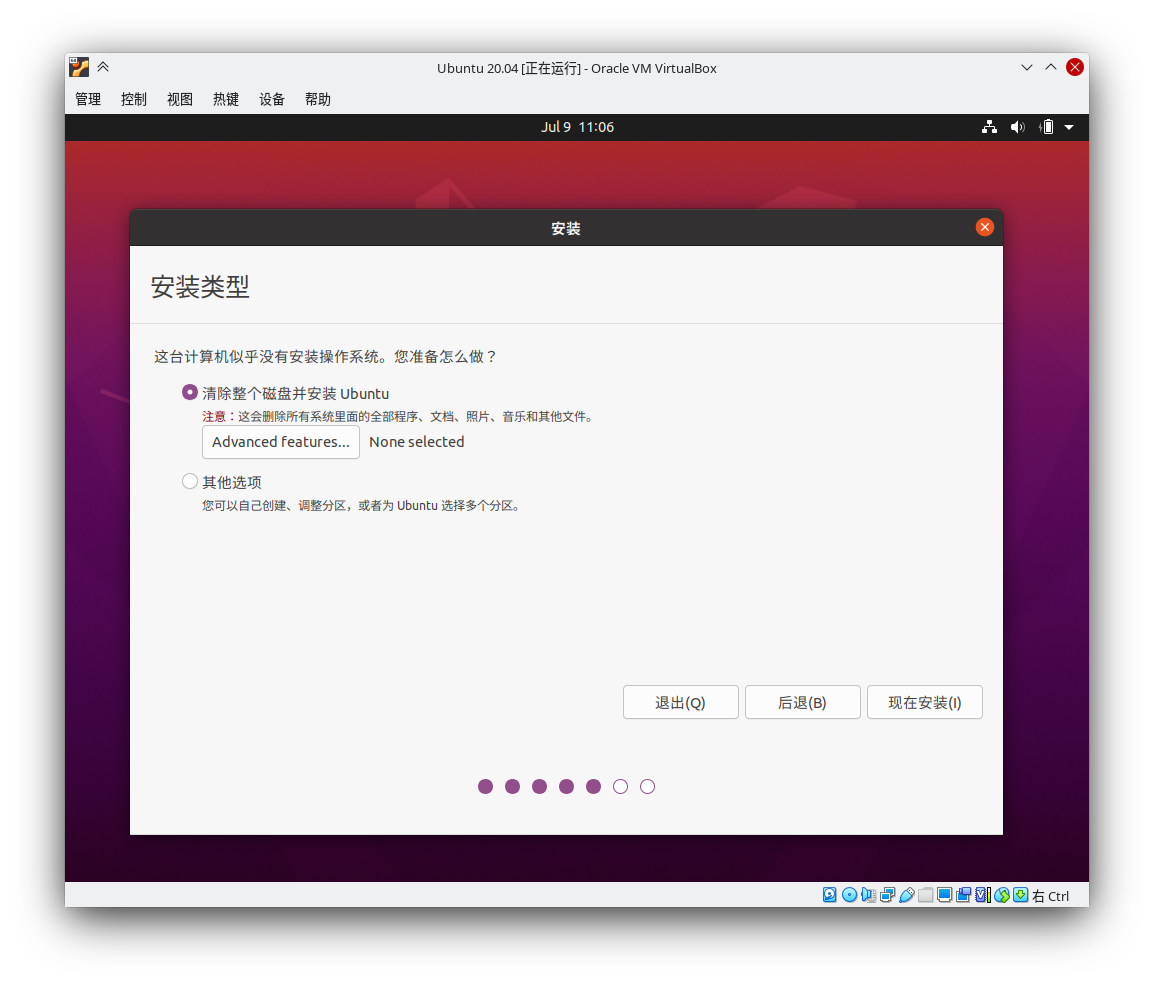
\includegraphics[width=0.7\textwidth]{fig/ubuntu_install_5.png}
					\caption*{安装类型}
				\end{figure}
			
				选择时区。
			
				\begin{figure}[H]
					\centering
					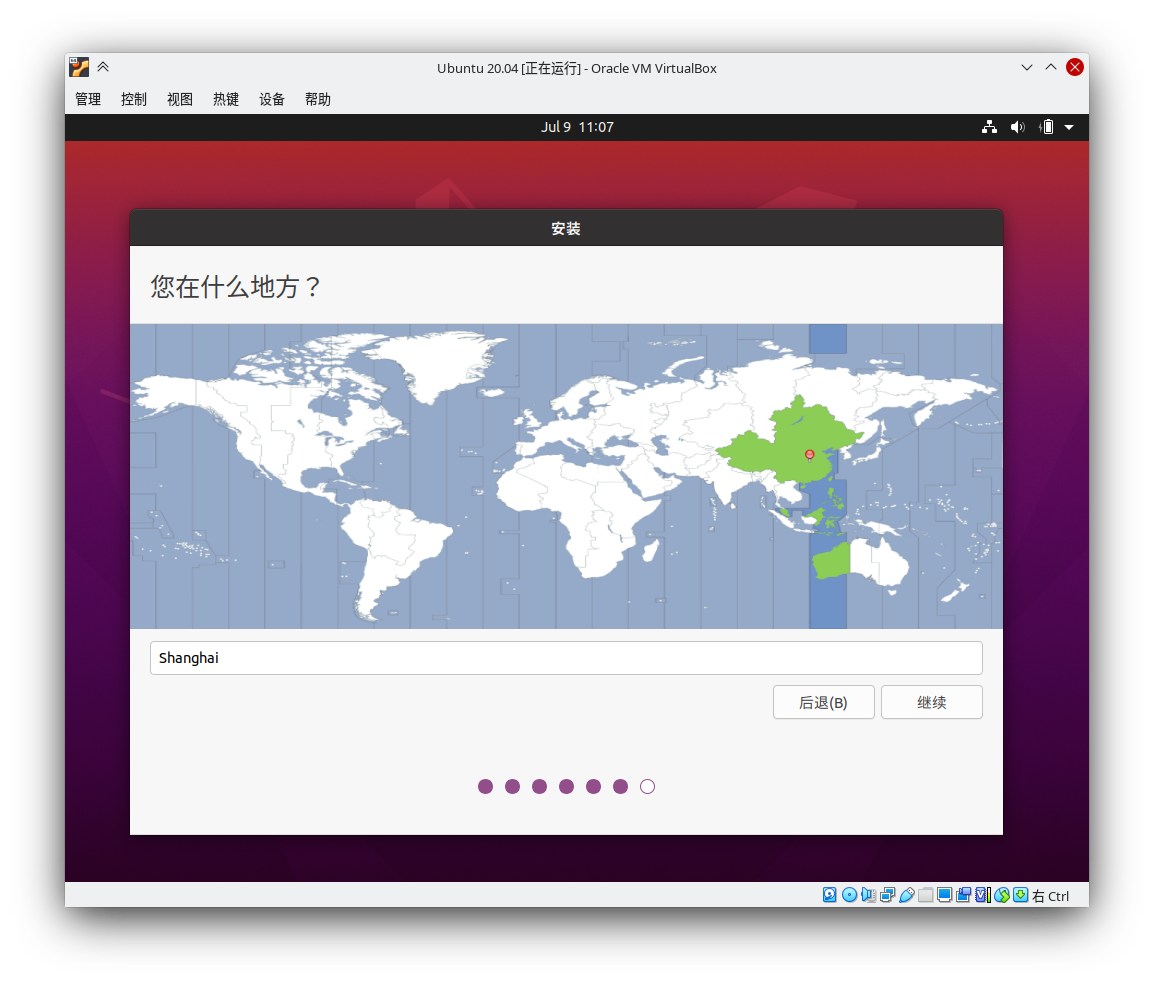
\includegraphics[width=0.7\textwidth]{fig/ubuntu_install_6.png}
					\caption*{选择时区}
				\end{figure}
			
				设置第一个用户。
				
				\begin{figure}[H]
					\centering
					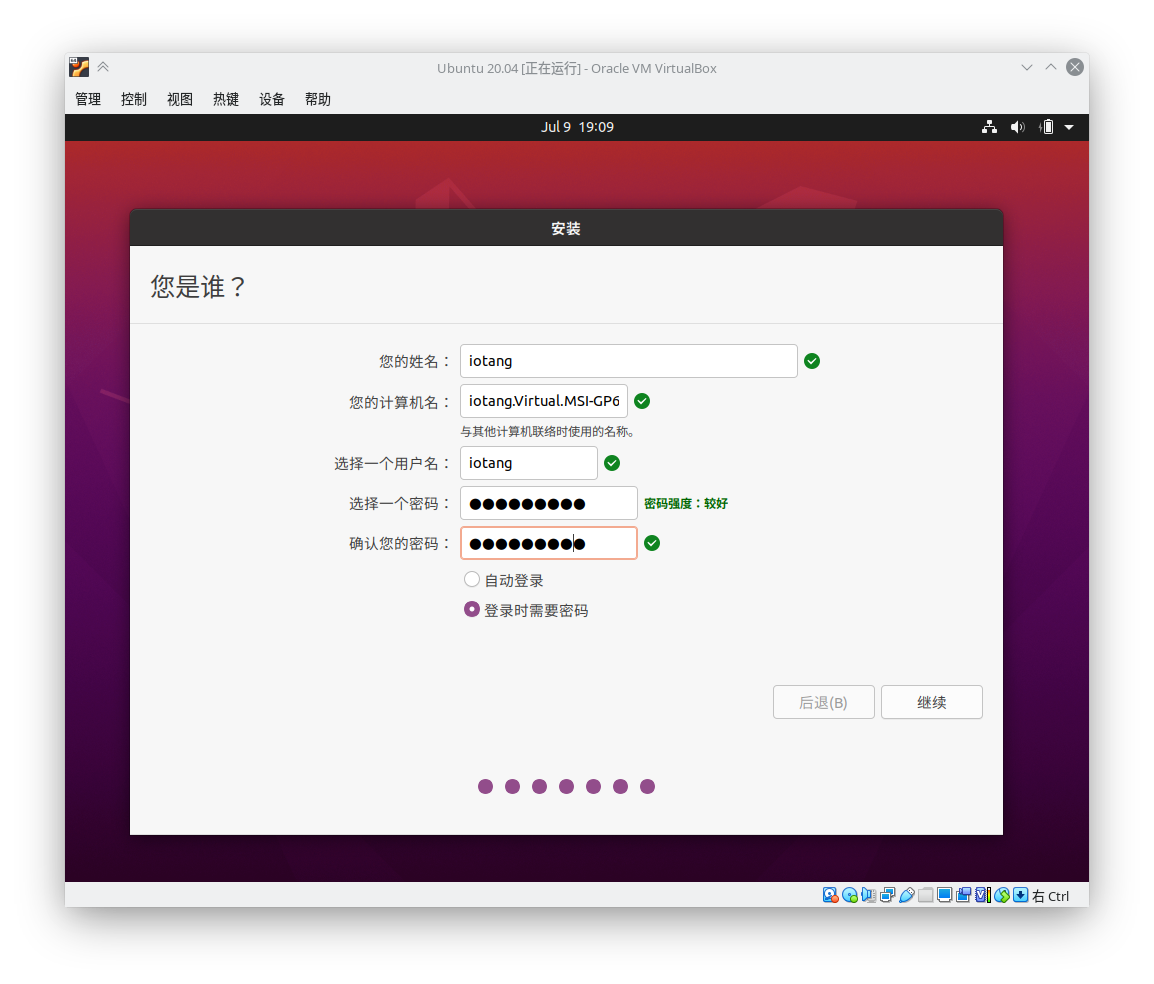
\includegraphics[width=0.7\textwidth]{fig/ubuntu_install_7.png}
					\caption*{我是中国弗兰常杀人}
				\end{figure}
			
				建议把网络关掉,以防安装程序用巨慢的速度下载一些东西,把安装时间拖得很长。
			
				\begin{figure}[H]
					\centering
					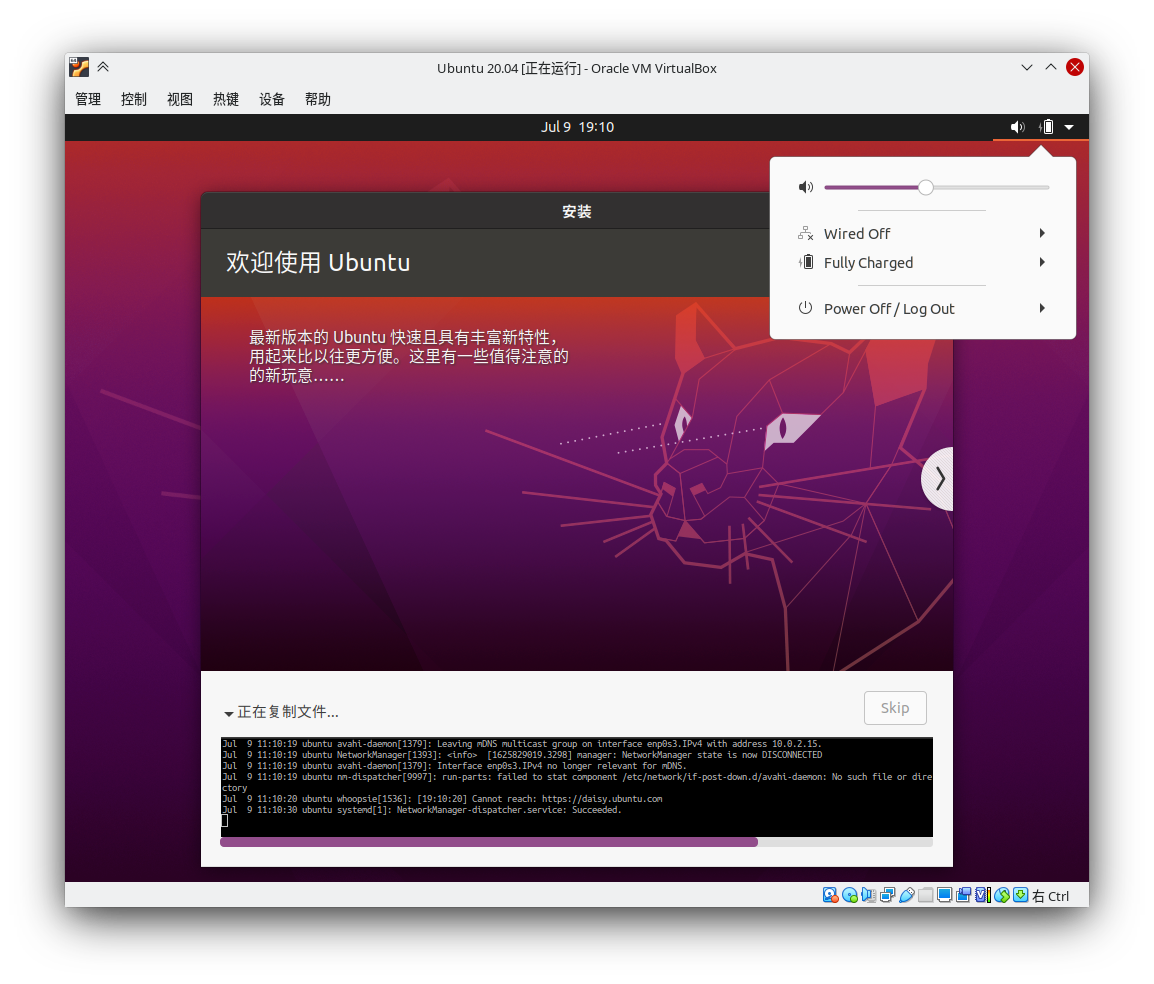
\includegraphics[width=0.7\textwidth]{fig/ubuntu_install_8.png}
					\caption*{关闭网络}
				\end{figure}
			
				之后关机,然后拔掉启动盘后开机。
				
				准备迎接 Ubuntu!第一次启动可能非常慢。
			
	\newpage
		
	\section{初始设置}
	
		\subsection{第一次更新软件}
		
			\subsubsection{软件源}
		
				更换 Ubuntu 的软件源到国内某一个,否则软件安装和更新的速度将非常慢,因为默认的源的地址不在国内。
				
				这边以清华大学开源软件镜像站为例子:
				
				百度到清华大学开源软件镜像站 Ubuntu 镜像使用帮助。
					
				\begin{figure}[H]
					\centering
					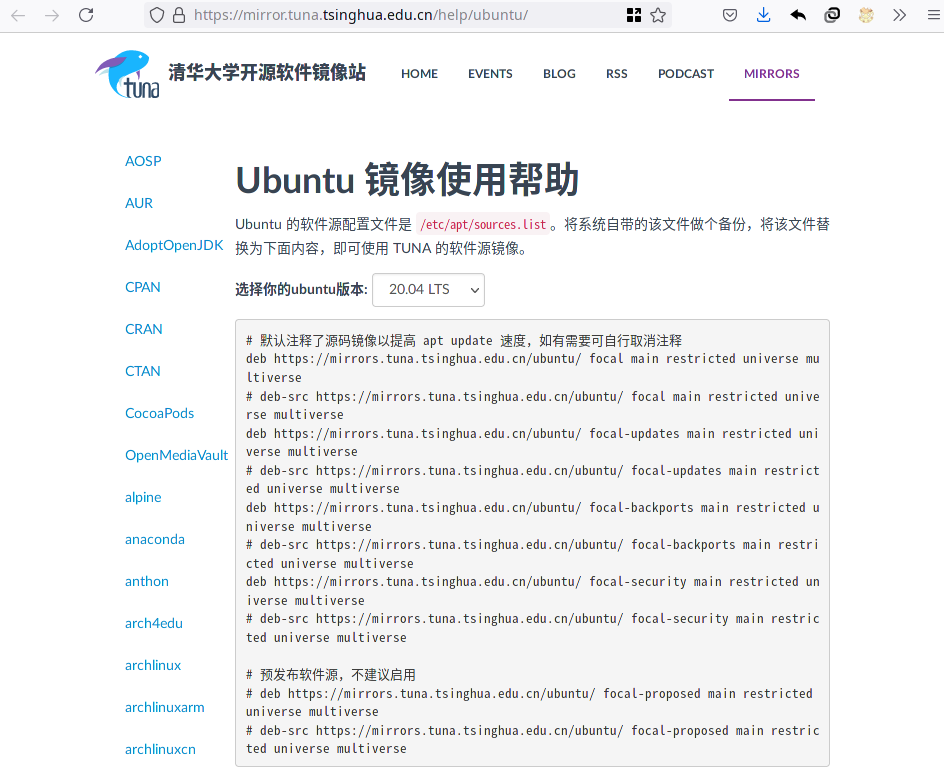
\includegraphics[width=0.8\textwidth]{fig/ubuntu_mirror_help.png}
					\caption*{贵校镜像站 Ubuntu 镜像使用帮助}
				\end{figure}
			
				选择正确的 Ubuntu 版本,复制镜像内容,然后编辑 \texttt{/etc/apt/sources.list}:
	
				\begin{minted}[frame=single]{console}
$ sudo gedit /etc/apt/sources.list
				\end{minted}
			
				(sudo 是以超级用户运行(后面的命令),即 \textbf{S}uper \textbf{U}ser \textbf{Do})
			
				(gedit 是 GNOME 桌面下的一个文本编辑器,即 \textbf{G}nome \textbf{Edit})
				
				从这里开始,以“\$”开头的东西代表你要在终端中执行这个语句(执行的语句里面没有“\$”)。比如对于上面那个命令,你可以先用快捷键 \texttt{Ctrl + Alt + T} 打开一个终端,然后输入 \texttt{sudo gedit /etc/apt/sources.list}(没有 “\$”):
	
				\begin{figure}[H]
					\centering
					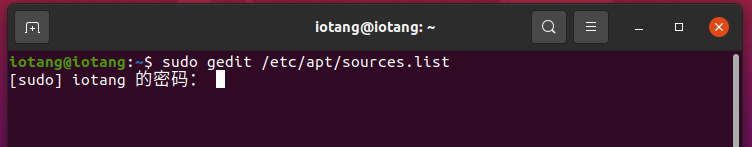
\includegraphics[width=0.8\textwidth]{fig/gedit_etcaptsourceslist.png}
					\caption*{打开 /etc/apt/sources.list}
				\end{figure}
				
				用你找到的镜像内容替换文件里原来的所有内容。
				
				\begin{figure}[H]
					\centering
					\begin{minipage}{0.38\textwidth}
						\centering
						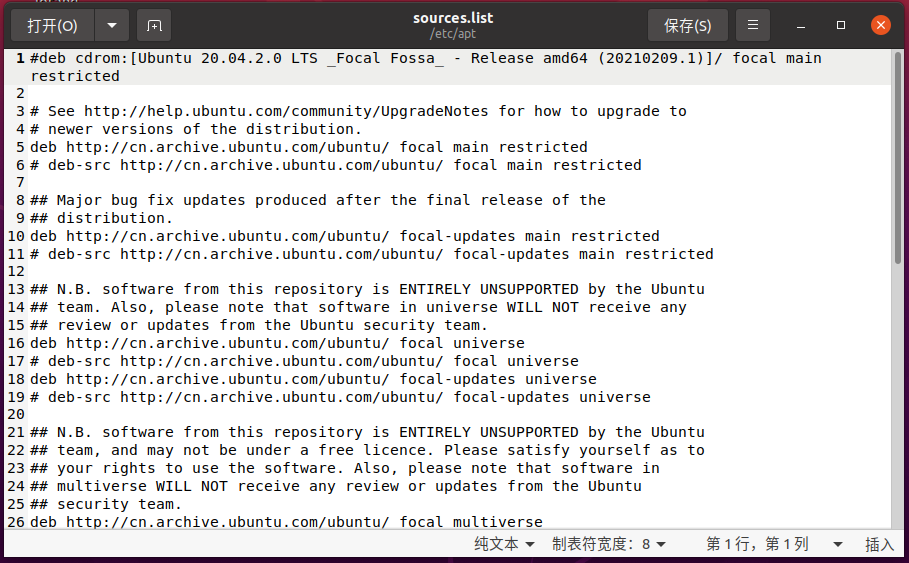
\includegraphics[width=\textwidth]{fig/sourceslist_before.png}
						\caption*{替换前}
					\end{minipage}
					\begin{minipage}{0.38\textwidth}
						\centering
						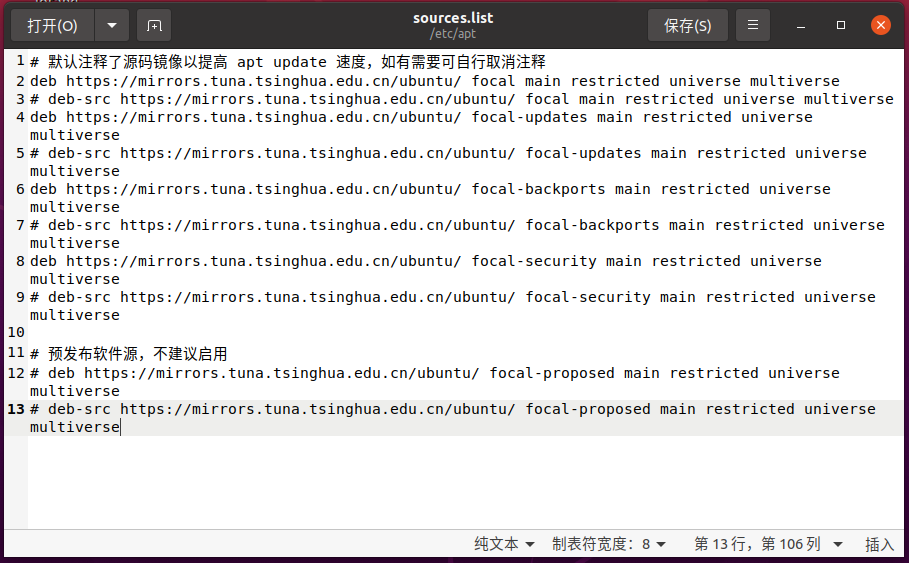
\includegraphics[width=\textwidth]{fig/sourceslist_after.png}
						\caption*{替换后}
					\end{minipage}
				\end{figure}
			
			\subsubsection{apt 是什么?}
			
				注意到了上文的 \texttt{/etc/apt/sources.list} 中的 apt 了吗?
	
				apt 是 Linux 下的安装包管理工具之一。Ubuntu 使用 apt。
				
			\subsubsection{更新软件列表}
				
				\begin{minted}[frame=single]{console}
$ sudo apt update
				\end{minted}
			
				更新软件列表可以让 apt 知道现在有哪些软件,以及那些软件的版本。
				
				apt 会将软件列表和目前的状况比对,然后就可以得出哪些软件可以更新。
				
				\begin{figure}[H]
					\centering
					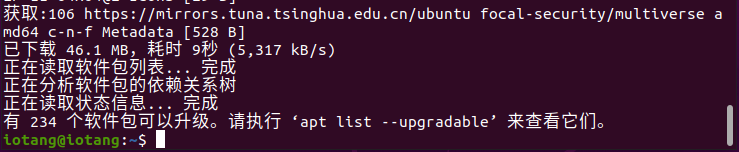
\includegraphics[width=0.8\textwidth]{fig/apt_update.png}
					\caption*{apt 找到了可以更新的软件}
				\end{figure}
			
			\subsubsection{更新软件}
	
				\begin{minted}[frame=single]{console}
$ sudo apt upgrade
				\end{minted}
				
				这可以让 apt 更新目前所有的软件。
				
				\begin{figure}[H]
					\centering
					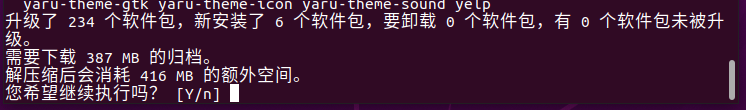
\includegraphics[width=0.8\textwidth]{fig/apt_upgrade_yn.png}
					\caption*{确定界面}
				\end{figure}
			
				在这里,[Y/n] 的 Y 是大写,意味着默认是“是”。也就是说,如果你在这里直接按下回车,那么就按“是”处理。
				
			\subsubsection{查找软件}
				
				\begin{minted}[frame=single]{console}
$ apt search xxx
				\end{minted}
			
				让 apt 在软件列表里查找相应字段。比如我想安装一个文本编辑软件 emacs:
				
				\begin{minted}[frame=single]{console}
$ apt search emacs
				\end{minted}

			\subsubsection{安装软件}
		
				\begin{minted}[frame=single]{console}
$ sudo apt install xxx
				\end{minted}
				
				比如我们刚才找到了 emacs 的软件名就叫 emacs,所以我们可以这样安装 emacs:
				
				\begin{minted}[frame=single]{console}
$ sudo apt install emacs
				\end{minted}
			
		\subsection{安装输入法}
		
			Linux 下想输入中文的话,一个方法是使用输入法。而搜狗输入法在 Linux 下仍然可用。
			
			百度到给 Linux 的搜狗输入法的主页:
		
			\begin{figure}[H]
				\centering
				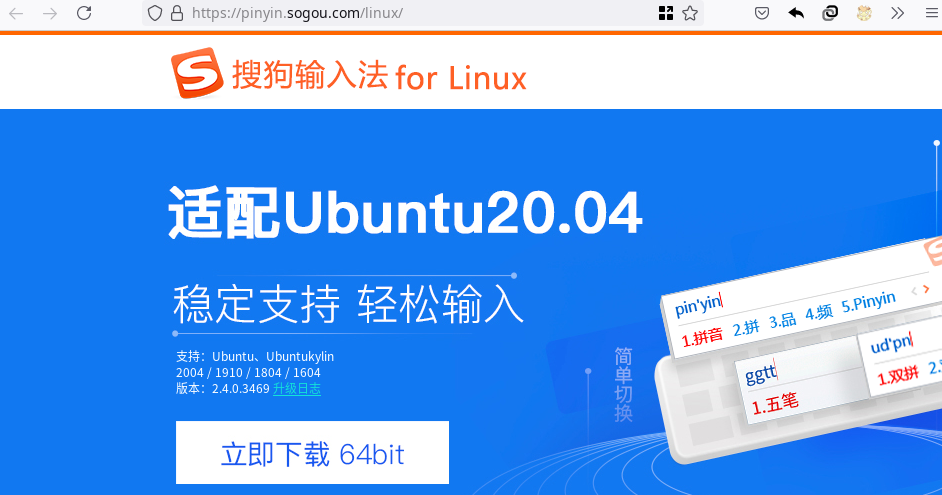
\includegraphics[width=0.8\textwidth]{fig/sogou.png}
				\caption*{搜狗输入法已经支持到了 Ubuntu 20.04}
			\end{figure}
	
			下载会得到一个以 .deb 结尾的安装包:sogoupinyin\_版本号\_amd64.deb。
			
			\subsubsection{添加中文语言支持}
			
				打开系统设置,找到“区域和语言”,点击“管理已安装的语言”。
				
				在“语言”栏下点击“添加或删除语言”。
				
				在弹出来的窗口里钩上“中文(简体)”,应用。
			
			\subsubsection{切换到 fcitx}
	
				回到“语言支持”窗口,在键盘输入法系统中,选择“fcitx”。
				
				如果没有 fcitx,那么把 fcitx 装上:
				
				\begin{minted}[frame=single]{console}
$ sudo apt install fcitx
				\end{minted}
			
			\subsubsection{安装搜狗输入法}
			
				直接双击打开这个安装包,在弹出的应用商店里安装。

\end{document}